\nnarticleheader{A Model of Shear-Induced Fibrillogenesis}{Dr. Holly M Golecki, Professor, University of Illinois at Urbana-Champaign}
Fibrillar proteins that support cells and tissues\textit{in vivo} are part of the extracellular matrix
(ECM). One ECM protein, fibronectin (FN), may play a significant role in organization, support
and development of the skin. In development, fetal skin contains high concentrations of FN.
These high expression levels also correspond with scarless healing after dermal injury. During
aging, highly elastic FN breaks down and is replaced by stiffer collagen. When a wound occurs
in adult skin, the healed tissue forms a dense collagen-rich ECM called a scar. We asked if
fibrillar FN applied to adult wounds could “trick” the microenvironment in assuming a fetal
phenotype and promote scarless healing in adults. This task presents a challenge as currently
available manufacturing techniques for protein fiber engineering have limited production rates.

\renewcommand{\thefigure}{1}
\begin{figure}[h]
  \begin{center}
    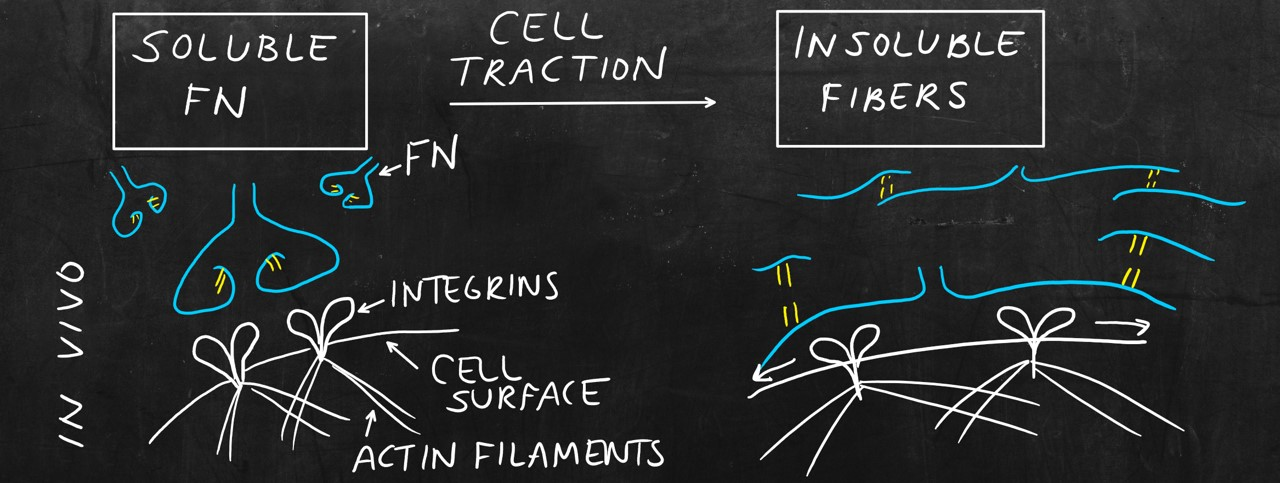
\includegraphics[width=\textwidth]{golecki_figure_1}
  \end{center}
  \caption{FN structure and unfolding in vivo. Schematic of the mechanism of FN fibrillogenesis.}
\end{figure}

To engineer fibrillar FN, we must first understand how it is built in vivo. Soluble,
globular FN circulates in the blood. Cells attach to FN via integrin binding receptors that transfer
mechanical traction forces to unfold FN. This unfolding exposes cryptic binding sites inducing
fibrillogenesis (Figure 1). The challenge is to replicate that process outside the body, turning fibrillogenesis into a manufacturing process. We propose that a perforated reservoir rotating at
high speeds may propel protein solutions out of the reservoir orifice stretching, drying and
solidifying nanofibers. Within that process we hypothesized that shear forces within the reservoir
are capable of unfolding FN inducing fibrillogenesis on the benchtop. Herein we describe a fluid
dynamics model of shear induced fibrillogenesis using this system to manufacture FN nanofibers
for future use in wound dressings.

\noindent
\textbf{Shear Fluid Model}

To test this hypothesis, we developed a mathematical model that predicts how shear forces generated using a spinning orifice can be used to induce the high-throughput production of FN nanofibers. Others have probed single FN molecules to determine tensile forces required to unfold FN. We used Mohr’s circle \cite{gere} to determine the shear stress required to unfold FN by translating values from single molecule uniaxial tensile tests \cite{oberhauser} to shear. Mohr’s circle is a graphical representation of the relationship between principle and shear stress. We calculated 3.7 kPa as the minimum shear stress required to unfold a FN molecule. Next, to calculate the shear produced by a spinning orifice, we derived a model from Navier Stokes for the shear stress distribution through the diameter of the orifice.

\renewcommand{\thefigure}{2}
\begin{figure}[h]
  \begin{center}
    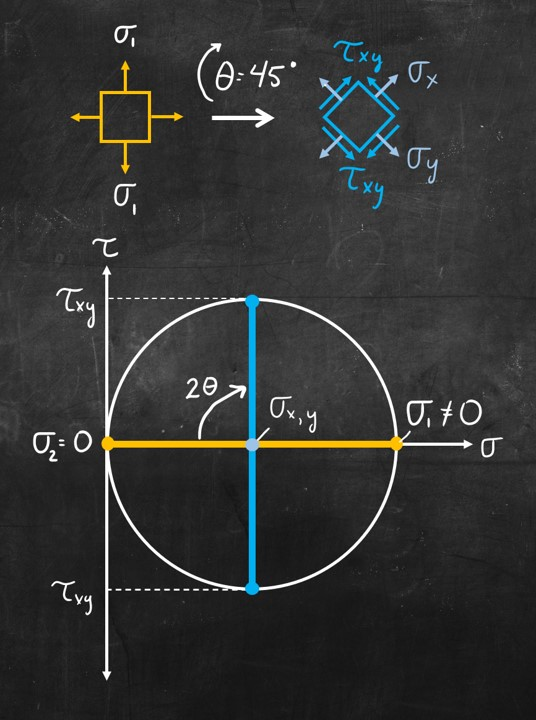
\includegraphics[scale=.55]{golecki_figure_2}
  \end{center}
  \caption{Mohr's circle for plane stress.}
\end{figure}

\renewcommand{\thefigure}{3}
\begin{figure}[h]
  \begin{center}
    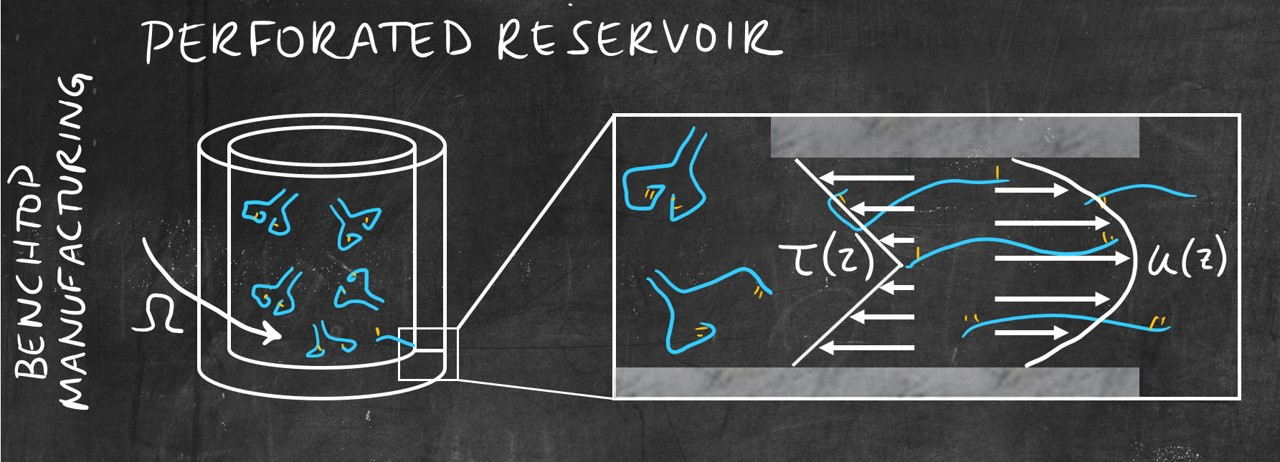
\includegraphics[scale=.5]{golecki_figure_3}
  \end{center}
  \caption{Schematic representing hypothesized benchtop shear unfolding in a rotating perforated reservoir.}
\end{figure}

\noindent
\textbf{Details of Shear Fluid Model}

To derive an equation of fluid flow through the orifice, we modeled shear stresses in a Poiseuille flow rotating with angular speed ($\Omega$). The system consists of a viscous, incompressible, fluid flowing through a tube of uniform cross section, rotating about the Y axis, applying the  following assumptions:

\begin{center}
1. The flow is steady and does not change with time: $\frac{du_z}{dt}=0$.\\
1a. Flow is in unidirectional: $u_r = 0; u_\theta = 0$.\\
2. The flow is axisymetric.
\end{center}

\renewcommand{\thefigure}{4}
\begin{figure}[h]
  \begin{center}
    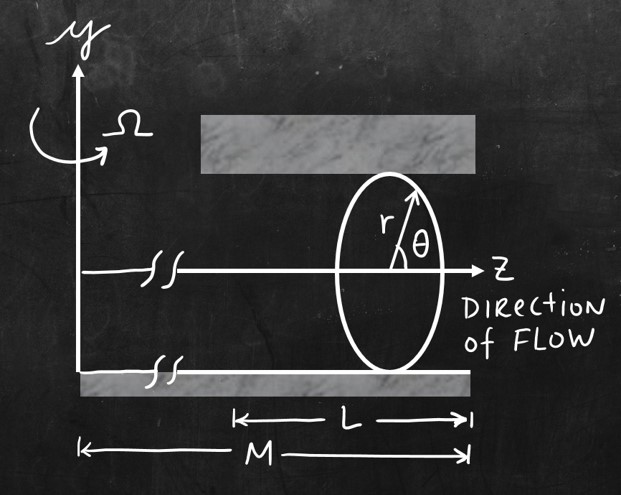
\includegraphics[scale=.42]{golecki_figure_4}
  \end{center}
  \caption{Schematic of reservoir orifice.}
\end{figure}

\noindent
\textit{Conservation of Mass (from the continuity equation):}
\[\frac{\partial}{\partial t}\rho 
+ \frac{1}{r}\frac{\partial r u_r}{\partial r}
+ \frac{1}{r}\frac{\partial r u_\theta}{\partial \theta}
+ \frac{\partial u_z}{\partial z}
= 0
\]

If density, $\rho$, does not change with time, there is no flow in the $r$ direction, then fluid speed does not change along the $z$ direction.
\[\frac{\partial u_z}{\partial z} = 0\]

\noindent
\textit{Conservation of Momentum:}

A very common case of Navier Stokes in cylindrical coordinates is axisymetric flow assuming no tangential velocity. The remaining quantities are independent of $\theta$. Therefore, N-S$_\theta$ goes to zero. Because we assume no flow in the $r$ direction, hydrostatic pressure is negligible, and $\frac{\partial u_z}{\partial z} = 0$ from continuity equation, N-S$_r$ goes to zero as well. From here, we study N-S in the $z$-direction:
\[z:(
\frac{\partial u_z}{\partial t}
+u_r\frac{\partial u_z}{\partial r}
+\frac{u_\theta}{r}\frac{\partial u_z}{\partial \theta}
+u_z\frac{\partial u_z}{\partial z})
= -\frac{\partial p}{\partial r}
+\mu(
\frac{1}{r}\frac{\partial}{\partial r}(
r\frac{\partial u_z}{\partial r})
+\frac{1}{r^2}\frac{\partial^2 u_z}{\partial \theta^2}
+\frac{\partial^2 u_z}{\partial z^2})
+\rho g_z
\]
The volumetric other body forces term, $\rho g_z$, is substituted with the volumetric centripetal force of rotation. Because $a = \Omega^2 r$, we replace the acceleration term with $\rho g \sim \rho \Omega^2 (z-M)$, with the assumption that $g<<\Omega^2 (z-M)$. We assume velocity does not change with time and velocity in the $r$ and $\theta$ directions is zero. The equation $\frac{\partial u_z}{\partial z} = 0$ above and the fact that we assume flow is axisymmetric, allows us to further simplify Navier Stokes$_z$ to:
\[0 = -\frac{\partial P}{\partial z}
+ \frac{\mu}{r}\frac{d}{dr}(
r\frac{du_z}{dr})
+\rho\Omega^2z
\]
Using Mathematics to solve for $u_z$ results in
\[u_z
= \frac{1}{4\mu}(
\frac{dP}{dz} - \rho\Omega^2(z-M))
r^2+c1\ln{r}+c2
\]
Pressure, $P=a_1+a_2z+a_3z^2$, simplifies to $\frac{\partial P}{\partial z} = a_2+2a_3$.
Next, we consider boundary conditions: $u_z$ is finite at $r=0$, $\ln{(0)}=1\rightarrow c_1=0$
From the continuity equation:
\[\frac{\partial u_z}{\partial z}
= 0 = \frac{\partial}{\partial z}
[\frac{1}{4\mu}(a_2+2a_3z-\rho\Omega^2z+\rho\Omega^2M)r^2+c_2]
\]
\[0=2a_3-\rho\Omega^2\]
\[a_3=\frac{1}{2}\rho\Omega^2\]
\[u_z=\frac{1}{4\mu}a_2 \cdot r^2 + c_2\]
Pressure Boundary Conditions at bottom and top of reservoir:
\[P_{bottom} = a_1+a_2M+\frac{1}{2}\rho\Omega^2M^2=\rho gh\]
\[P_{top}=a_1+a_2(M+L)\frac{1}{2}\rho\Omega^2(M+L)^2 = 0\]
Subtract $P_{top}-P_{bottom}$
\[a_2=-\frac{\rho gh}{L} - \rho\Omega^2M-\frac{1}{2}\rho\Omega^2L\]
No slip boundary conditions at the pipe wall requires $u_z(r=R)=0$
\[c_2 = \frac{1}{4\mu}(\frac{\rho gh}{L}-\rho\Omega^2M-\frac{1}{2}\rho\Omega^2L)R^2\]
\[u_z=\frac{1}{4\mu}(\frac{\rho gh}{L}+\rho\Omega^2M+\frac{1}{2}\rho\Omega^2L)(R^2-r^2)\]
\[u_z=\frac{\rho}{8l\mu}(2gh+2\Omega^2ML+\Omega^2L^2)(R^2-r^2)\]
The shear stress is generally defined as:
\[\tau(r)=\mu\frac{du_z}{dr}\]
and specifically as:
\[\tau(r)=(-\frac{\rho}{4L}(2gh+2\Omega^2ML+\Omega^2L^2)r)\]
Hydrostatic pressure $\frac{dp}{dz}\sim\frac{\Delta p}{\Delta z} = -|\frac{\Delta p}{\Delta z}|$
\[\tau(r)\propto R\]
\[\tau(r)\propto \Omega^2\]
Hydrostatic pressure is negligible compared to centripetal pressure due to reservoir spinning with $\rho_{FN solution}\sim 1600\frac{kg}{m^3},g=9.8\frac{m}{s^2},h\sim 0.1m.$
\[P_{hydrostatic\,@\,bottom\,of\,res.} = \rho gh 
= (1600\frac{kg}{m^3})
(g=9.8\frac{m}{s^2})
(0.1m)
= 156.8\,Pa
\]
\[P_{centripetal} = \rho z\Omega^2
= (1600\frac{kg}{m^3})
(0.01m)^2
(333\frac{1}{s})^2
= 17742\,Pa
\]
The below equation gives the shear stress distribution, $\tau(r)$, that scales linearly with distance from the center and is dependent on rotation speed,
\[\tau(r)=(-\frac{\rho}{4L}(2gh+2\Omega^2ML+\Omega^2L^2)r)\]
where $\rho$ is protein solution density, $L$ is orifice length, $\mu$ is dynamic viscosity, $h$ is reservoir height, $\Omega$ is rotation speed, $M$ is reservoir radius, and $r$ is orifice radius. Calculated shear stresses achievable within the spinning reservoir ranges from $0-30\,kPa$. This range of fluid shear stress is achieved through a combination of high rotation speeds ($\sim 30000\,rpm$) and small orifice geometries ($\sim 400\mu m$ diameter).  

\renewcommand{\thefigure}{5}
\begin{figure}[h]
  \begin{center}
    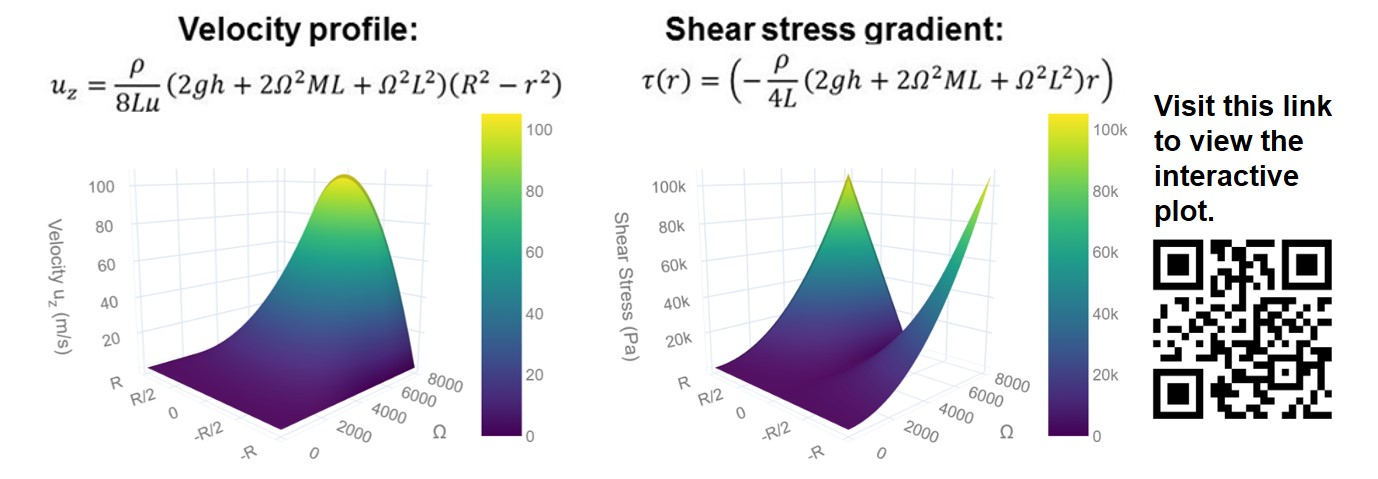
\includegraphics[width=\linewidth]{golecki_figure_5}
  \end{center}
  \caption{Visualization of fluid shear model within the orifice of a spinning reservoir.}
\end{figure}

\noindent
\textbf{Conclusion}

In addition to shear forces unfolding the FN molecules and inducing fibrillogenesis, it may be possible to modulate the degree of unfolding with applied shear. Our model indicates that by increasing rotation speed from $25,000rpm$ to $75,000rpm$, you increase the shear and achieve a negligible difference in percentage unfolding, but with increasing shear there is an increasing extent of unfolding. This makes it possible to spin FN solutions, at two spinning speeds and achieve fibers with different degrees of folded untrastructure. 

It is well understood that the ECM recruits and stabilizes growth factors. Within a wound site, the ECM can concentrate growth factors to promote healing \cite{sawicka}. Beyond simply acting as a reservoir for growth factors, ECM proteins can modulate the activity of growth factors. FN can enhance the activity of growth factors via cryptic binding sites that become exposed when the protein fibrils are under cellular tension \textit{in vivo}. For example, VEGF, a growth factor important for vascularization of regenerated skin, attaches to one exposed FN binding site and one cryptic site along the molecule \cite{sawicka}. Within the folded FN domains, FN peptide, P12, can bind platlet derived growth factor with high affinity. As lab scale production of FN is explored, what role can mechanical stretch play in tuning biological activity to improve wound healing? Can FN fibers spun at high speeds in RJS bind growth factors with higher affinity than those at low speeds? Can FN fibers be produced with higher affinity for growth factor binding than naïve fibers further enhancing the wound healing capabilities of FN fibrils and wound dressings? The shear model presented here provides a tool to explore the mechanochemical properties of engineered proteins.

Article adapted from Golecki, H. (2018) From Design to Production: Applications of Polymer and Protein Nanofibers for Regenerating Tissue. Ph.D. Dissertation. Harvard University.

\noindent
\textbf{References}
\begingroup
\renewcommand{\section}[2]{}% https://tex.stackexchange.com/questions/22645/hiding-the-title-of-the-bibliography
%\renewcommand{\chapter}[2]{}% for other classes
\begin{thebibliography}{3}
\bibitem{gere}
Gere, J. M. (2003). Mechanics of Materials: Thompson-Engineering.

\bibitem{oberhauser}
Oberhauser, A. F., Badilla-Fernandez, C., Carrion-Vazquez, M., and Fernandez, J. M. (2002).
The mechanical hierarchies of fibronectin observed with single-molecule AFM. 
\textit{Journal of Molecular Biology}, 319(2), 433-447. doi:10.1016/s0022-2836(02)00306-6

\bibitem{sawicka}
Sawicka, K. M., Seeliger, M., Musaev, T., Macri, L. K., and Clark, R. A. (2015). Fibronectin
interaction and enhancement of growth factors: importance for wound healing. 
\textit{Advances in wound care}, 4(8), 469-478.

\end{thebibliography}